\documentclass[12pt,twoside]{article}

% Things that are not loaded by the package, though these might be
% generally useful.
\usepackage{natbib}
\usepackage{graphicx}
\setcounter{secnumdepth}{0}

\usepackage{amsthm}

\renewcommand\thefigure{S.\arabic{figure}}
\renewcommand\thetable{S.\arabic{table}}

% Load the package first - should sort everything out...
\usepackage{suppmat}

% ...and then we add some metadata
\titleprefix{Supplemental Material}
\runninghead{Y fuse?}
\title{Y fuse? Sex chromosome fusions in fishes and reptiles}
\author{Jun Kitano$^1$, Matthew W. Pennell$^2$, Mark Kirkpatrick$^3$,\\ Sarah P. Otto$^4$, Jana C. Vamosi$^5$, \& Catherine L. Peichel$^6$}
\address{
1& Ecological Genetics Laboratory, National Institute of Genetics, Mishima, Shizuoka 411-8540, Japan\\
2& Institute for Bioinformatics and Evolutionary Studies, University of Idaho, Moscow, ID 83844, USA\\
3& Department of Integrative Biology, University of Texas, Austin, TX 78712, USA\\
4& Department of Zoology, University of British Columbia, Vancouver, BC V6J 3S7, Canada\\
5& Department of Biological Sciences, University of Calgary, Calgary, AB T2N 1N4, Canada\\
6& Divison of Human Biology, Fred Hutchinson Cancer Research Center, Seattle, WA 98109, USA\\}
\emailaddress{\email{jkitano@lab.nig.ac.jp}}
\date{}

\begin{document}

\maketitle

\section{Details of phylogenetic analyses}

To investigate the relative rates of different types of fusions across our two focal groups--teleost fishes and squamate reptiles--we fit multiple phylogenetic models to our karyotype dataset. We first matched the available karyotype data to the fish \citep{Rabosky2013} and squamate \citep{squamatetree, PyronBurbrink2014} phylogenies (using an approximate matching algorithm described in the main text). This resulted in phylogenetic comparative datasets containing 163 species of fish and 261 squamate species.  We conducted two separate types of analyses on both groups. First, we examined differences between XY and ZW systems; here, we treat X-autosome and Y-autosome fusions as equivalent (and likewise, Z-autosome and W-autosome fusions). Results from this first analysis are presented in the main text. Second, we investigated autosomal fusion rates for all types of sex chromosomes individually (i.e., Y, X, W, and Z autosome fusions). While the second analysis provides more detailed resolution, the low numbers for some of the fusions made it difficult to reliably estimate rates. All analyses were done using the R package \textsc{diversitree} \citep{FitzJohn2012} and code to reproduce all results can be found at \texttt{https://github.com/mwpennell/fuse/analysis}. 

\subsection{Fusion rates in XY vs. ZW systems}

The most general model for transition rates was a Markov model \citep{Pagel1994} with the following states
\begin{itemize}
\item[$XY$] Male heterogametic unfused
\item[$XY_F$] Male heterogametic fused (XXY or XYY)
\item[$ZW$] Female heterogametic unfused
\item[$ZW_F$] Female heterogametic fused (ZZW or ZWW)
\end{itemize}
where transitions between all states were allowed. We use the notation $q_{A.B}$ to represent the transition rate between states $A$ and $B$. We used likelihood ratio tests to restrict the model in order to improve our ability to estimate the parameters of interest. We first imposed the biologically reasonable constraint that prior to becoming $XY_F$ (or $ZW_F$), a lineage must first be $XY$ (or $ZW$); e.g., the transition rate from female heterogametic unfused to male heterogametic fused $q_{ZW.XY_F}$ was set to be 0. 

Next, we proposed a model in which the rate of sex chromosome turnover--going from a XY to a ZW system and \emph{vice versa}--did not depend on whether the lineage contained a fused sex chromosome or not (e.g., $q_{XY_F.ZW} = q_{XY.ZW}$). In both fish and squamtes, this restriction was acceptable.

In the next step, we proposed a model in which the rate of chromosomal fission, going from a fused sex chromosome system to an unfused system of the same type, was the same for XY and ZW systems. In fish, a likelihood ratio test favored the more restricted model, where as in squamates, the more general model (where $q_{XY_F.XY} \neq q_{ZW_F.ZW}$) was favored ($p=\text{0.012}$). The support for the more general model in squamates resulted from our inability to reliably estimate the transition rate from fused female heterogametic to unfused female heterogametic $q_{ZW_F.ZW}$, owing to the scarcity of ZW fusions in the data. We therefore took slightly different approaches when analyzing the two clades.

For fish, we simply compared the restricted model (where $q_{XY_F.XY} = q_{ZW_F.ZW}$) to a model in which the XY and ZW fusion rates were set to be equal ($q_{XY.XY_F}=q_{ZW.ZW_F}$) to test whether the two rates were siginficantly different. We found the rate difference to be highly significant ($p=\text{0.014}$) using a likelihood ratio test. To better accomodate uncertainty in the estimate, we ran a Bayesian analysis (described in the text) and this too was unequivocal in supporting our hypothesis that XY fusions occur at a higher rate than ZW fusions (98.6\% of the posterior probability supported this and the 95\% Credible Interval for the difference in rates did not overlap with 0; Figure 4 in the main text).

For the squamate data, we took two tacts. First, we went forward assuming that the `equal fission rates model' was indeed reasonable and as with the fish, restricted the model even further to test for a difference in the rates of fusion between XY and ZW systems. Using a likelihood ratio tests, the difference was found to be highly significant ($p=\text{0.003}$). The same was true for the Bayesian analysis (99.9\% of the posterior probability distribution supported this conclusion; Figure 4 in the main text). Second, we used a Bayesian MCMC to fit a model in which $q_{ZW_F.ZW}$ was estimated independently of $q_{XY_F.XY}$. For this model the support for the difference between $q_{XY.XY_F}$ and $q_{ZW.ZW_F}$ was not as strong (92.0\% of the posterior probability supporting $q_{XY.XY_F} > q_{ZW.ZW_F}$; Figure \ref{fig:squa-dif}).

\begin{figure}[p]
\centering
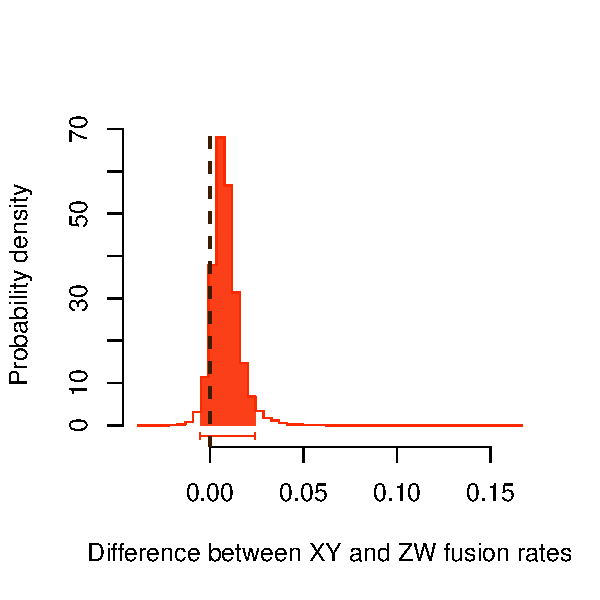
\includegraphics[scale=1.25]{figs/karyotype-fusion-squa-6par}
\caption{Posterior estimate of the rate difference between XY and ZW fusions in squamate reptiles when we estimate the fission rates $q_{XY_F.XY}$ and $q_{ZW_F.ZW}$}
\label{fig:squa-dif}
\end{figure}

However, the transition rate may be misleading when the reverse parameters are difficult to estimate. If there are very few or no `observed' fission events in one state, this pattern could be explained by either a very low rate of fission or else a very high rate of fission, such that any fusions that did occur reverted back immediately and would likely be missed. We therefore examined the
residency time of the various states. Rather than examine the transition rates from unfused to fused states, we asked whether XY fusions were more evolutionarily stable than ZW fusions. The residency time $q_R$ for XY fusions can be computed as
\begin{equation}
q_{R,XY_F} = \frac{q_{XY.XY_F}}{(q_{XY.XY_F} + q_{XY_F.XY})}
\end{equation}
And likewise, $q_{R,ZW_F}$ is
\begin{equation}
q_{R,ZW_F} = \frac{q_{ZW.ZW_F}}{(q_{ZW.ZW_F} + q_{ZW_F.ZW})}
\end{equation}

Using a Bayesian analysis, we found very strong support for the residency time being greater for XY fusions than ZW fusions (99.8\% of the posterior probability supported $q_{R,XY_F} > q_{R,ZW_F}$; Figure \ref{fig:squa-resid}). While there are different limitations to each of these analyses, the fact that they all point towards the same conclusions gives us greater confidence in the results.

\begin{figure}[p]
\centering
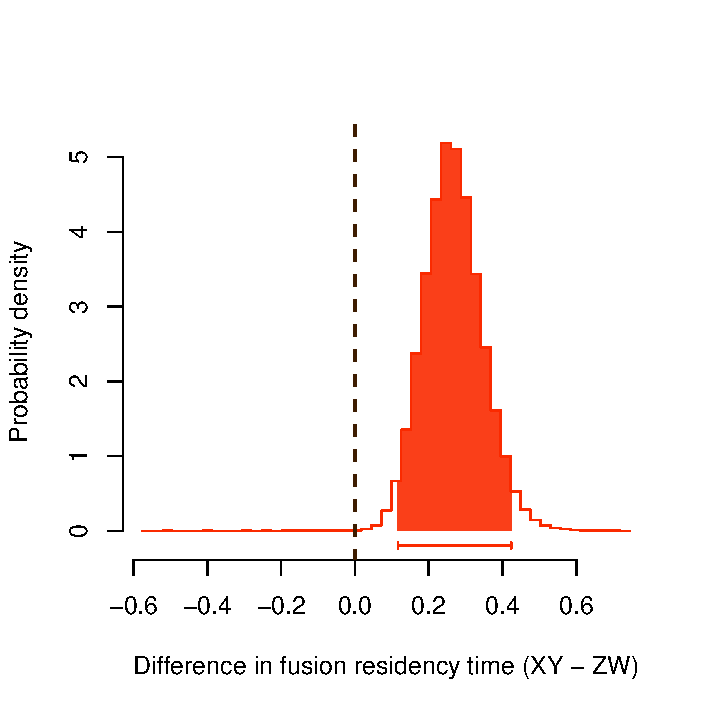
\includegraphics[scale=1.1]{figs/karyotype-residency-squa-6par}
\caption{Posterior estimate of the difference in residency time between XY and ZW fusions (i.e., $q_{R,XY_F} - q_{R,ZW_F}$) in squamate reptiles.}
\label{fig:squa-resid}
\end{figure}


\subsection{Comparing fusion rates between chromsomes} 

Rather than classifying the states as male/female heterogametic unfused/fused, we separated out the different types of fusions (i.e., classifying X-autosome [XA] and Y-autosome [YA] fusions as being different states). This allowed us to assess whether the patterns we observed were driven by an overabundance of autosomal fusions with the Y chromosome. After matching the data to the tree, we did not have any records of WA fusions in fish and in squamates, there were no observed any XA fusions.

For both the fish and the squamates, we again restricted the model via a nested series of likelihood ratio tests. For both clades, we found it to be statistically justifiable to assume that: a) transitions from one fused state to another fused state were impossible; b) prior to becoming fused, a lineage had to be in the corresponding unfused state; and c) fission rates were constrained to be equal. This allowed us to reliably evaluate whether the fusion rates differed by chromosome.

For the fish, using likelihood ratio tests, we found YA fusions to be significantly higher than XA fusions ($p=\text{0.016}$) and ZA fusions ($p=\text{0.035}$). XA and ZA fusion rates were not significantly different ($p=\text{0.658}$). Again, WA fusions did not exist in the fish analysis so we could not compare them to other classes. We then performed a Bayesian MCMC analysis to gain a better estimate of the relevant parameters. For the purposes of this analysis, we fixed XA and ZA fusions to occur at the same rate and then compared the YA fusion. We found that YA fusions occur at a much higher rate than XA/ZA fusions (Figure \ref{fig:fish-ind}; 99.5\% of the posterior distribution supported this conclusion).

\begin{figure}[p]
\centering
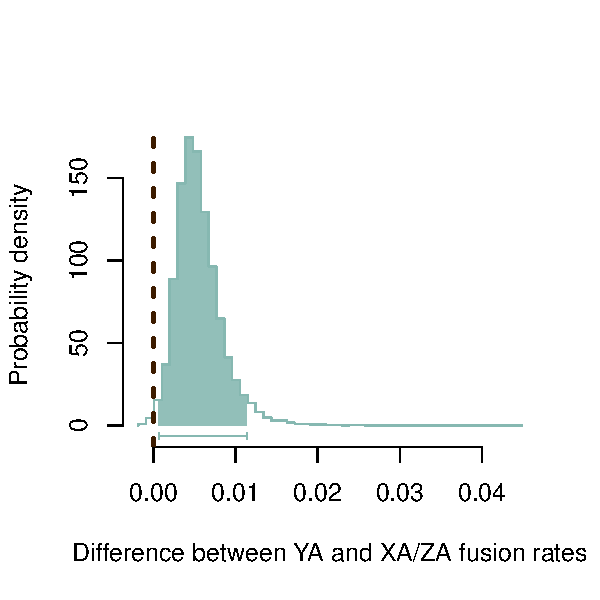
\includegraphics[scale=1.25]{figs/chromosome-fusion-fish}
\caption{Posterior estimate of the rate difference between YA and XA/ZA fusions in fish. When the estimate is greater than 0, this means that the YA fusion rates are higher than those of the other chromosomes}
\label{fig:fish-ind}
\end{figure}

For the squamate analysis, YA fusions also occured at a higher rate than WA fusions ($p<\text{0.001}$) and ZA fusions ($p<\text{0.001}$). WA and ZA fusions rates were not significantly different from one antoher ($p\approx \text{1}$). As with the fish, for the Bayesian analysis we set WA and ZA fusion rates to be equal and estimated the difference between YA fusions and other type of fusions. 99.9\% of the posterior probability distribution supported YA fusions occuring at a higher rate than fusions on other chromosomes (Figure \ref{fig:squa-ind}). 

Taken together, these results strongly suggest that the difference between XY and ZW fusion rates is driven almost entirely by the very high rates of autosomal fusions with the Y relative to the other sex chromosomes.

\begin{figure}[p]
\centering
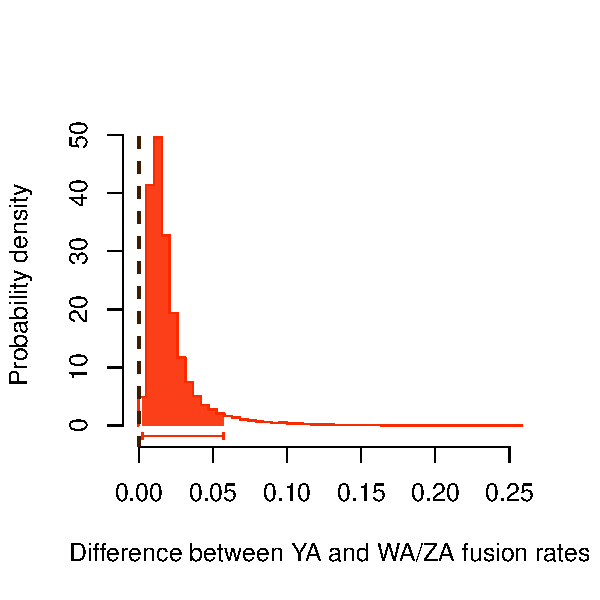
\includegraphics[scale=1.25]{figs/chromosome-fusion-squa}
\caption{Posterior estimate of the rate difference between YA and WA/ZA fusions in squamate reptiles. When the estimate is greater than 0, this means that the YA fusion rates are higher than those of the other chromosomes}
\label{fig:squa-ind}
\end{figure}

\clearpage
\bibliographystyle{sysbio}
\bibliography{suppmat.bib}

\end{document}
